\chapter{Epipolar Geometrie}
\label{sec:epipolar} 

\textcolor{red}{Epipolar geometry is central to stereovision. On the one hand, knowing
	it enables to strongly constrain the problem of matching two images.
	On the other hand, it can be estimated from matches and then allows
	for motion estimation, self-calibration, and triangulation of 3D points
	or other geometric primitives.\cite{CamerModels.}}

Epipolargeometrie beschreibt ähnlich der Homographie eine Beziehung der projektiven Geometrie zwischen zwei Bildern\cite{HZ}.

Epipolargeometrie beschreibt eine intrinsische projektive Geometrie zwischen zwei Bildern\cite{HZ}. Sie dient insbesondere zur Korrespondenzanalyse von Punkten aus Bildern und zur Gewinnung von 3-D-Informationen. 

Ohne Kenntnis der Kamerapositionen, kann mit Hilfe der Epipolargeometrie eine einfache Beziehung zwischen korrespondierenden Punkten hergestellt werden. Abbildung 3.12 zeigt, den Aufbau zweier Kameras mit ihren Projektionszentren $C$ und $C'$, deren Bildebenen $I$ und $I'$, welche vor den Projektionszentren platziert wurden. Die Bildebenen können sich auch hinter den Projektionszentren befinden, das hat letztendlich keinen Einfluss auf die geometrischen Beziehungen\cite{HZ}. Zu den Elementen der Epipolargeometrie gehören zum einen die Epipole $e$ und $e'$. Betrachtet man die Basislinie zwischen den beiden Projektionszentren, so entsteht der Epipol genau am Schnittpunkt der Verbindungslinie mit den jeweiligen Bildebenen. Tritt der Fall ein, dass die Basislinie parallel zu einer oder beiden Bildebenen ist, so kommt es zu keiner Abbildung des Epipols auf den entsprechenden Bildebenen, sondern der Epipol befindet sich in diesem Falle im unendlichen\cite{ZZGXr}. Das hat zur Folge, dass alle Epipolarlinien, welche durch den Epipol verlaufen, sich zueinander parallel anordnen. Epipolarlinien die Linien, welche durch einen Bildpunkt $m$ oder $m'$ und dem jeweiligen Epipol $e$ oder $e'$ des Bildes verlaufen. Der Korrespondierende Punkt zu $m$ ist $m'$ und die korrespondierende Epipolarlinie $l'$ zu $m$, ist diejenige Linie, welche durch $m'$ und $e'$ verläuft. 


\begin{minipage}{\linewidth}
	\centering
	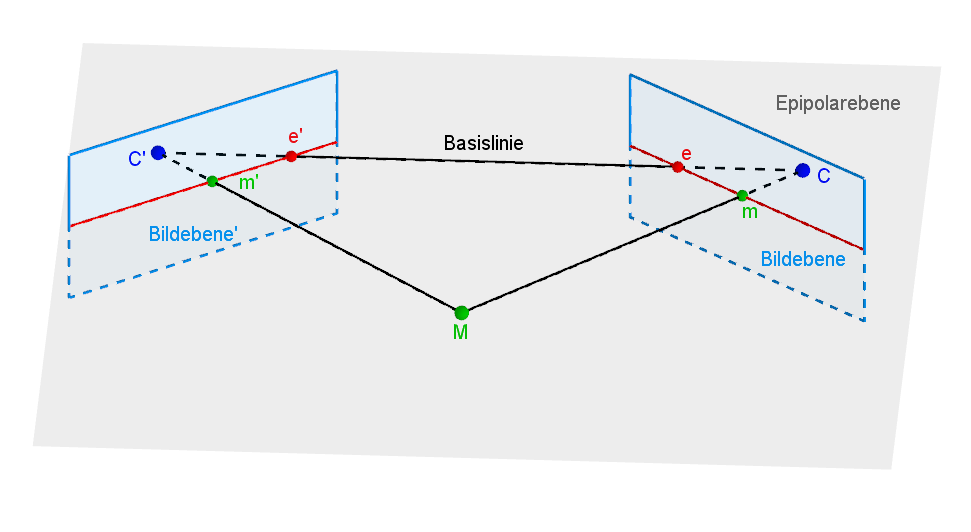
\includegraphics[width=1.\linewidth]{images/EpipolarGeoemtrieGrafik.png}
	\captionof{figure}{Grafik zu den geometrischen Eigenschaften der Epipolargeometrie zwischen zweik Bildern. $C$ und $C'$ sind die Projektionszentren zweier Kameras. Beide Kameras besitzen jeweils eine Bildebene. Die Basislinien verbindet die Projektionszentren der Kameras. Der Punkt an welchem die Basislinie die Bildebenen schneidet, wird als Epipol bezeichnet. Durch den Epipol verlaufen alle Epipolarlinien des Bildes. $M$ ist der Objektpunkt im 3D-Raum und $m_1$ und $m_2$ sind die jeweiligen Abbildungen dieses Punktes auf den Bildebenen. Die Verbindungsvektoren zwischen $C, C'$ und $M$ bilden die sogenannte Epipolarebene\cite{Elements,HZ,ZZGXr}.}  
	\label{fig:Epipolargeometry}
\end{minipage}\\ \\


Die Epipolarlinie $l'$, beinhaltet alle möglichen korrespondierenden Punkte zu $m$. Wenn $C$ auf seiner Bildebene $I$ einen Punkt $m$ abbildet, so erscheint dieser Punkt immer an der selben Stelle auf dem 2D - Bild, egal wie nah der Ursprüngliche 3D-Objektpunkt $M$ an $I$ befindet. Rein theoretisch, könnte der Originial Szenenpunkt $M$, sich überall auf der Verbindungslinie $\overline{Mm}$ befinden. Der Abgebildete Punkt $m$ wäre auf $I$ immer an der selben Stelle abgebildet. Fährt man nun mit $M$ die Verbindungslinie $\overline{Mm}$ entlang, dann ist $m$ immer an der selben Stelle auf $I$ zu sehen, während der korrespondierende Punkt $m'$ sich entlang der Epipolarlinie bewegen würde. Die Epipolargeometrie beschreibt also eine Beziehung zwischen einem Bildpunkt $m$ und dessen korrespondierender Epipolarlinie $l'$, welche wiederum alle möglichen zu $m$ korrespondierenden Punkte $m'$ beinhaltet\cite{HZ,Zhang2014,ZZGXr}.\\



\begin{minipage}{\linewidth}
	\centering
	\includegraphics[width=1.\linewidth]{images/EpipolarLinien.png}
	\captionof{figure}{Die Objektpunkte $M_1, M_2$ und $M_3$ werden in $I'$ als $m'_1, m'_2$ und $m'_3$ abgebildet, während sie in $I$ immer den selben Bildpunkt $m_1$ ergeben.}  
\end{minipage}\\ \\


Die Epipolargeometrie lässt sich, ähnlich wie eines Homographiematrix, in einer 3x3-Matrix zusammenfassen. Diese ist jedoch singulär und besitzt somit nicht wie die Homographiematrix Rang 3 sondern Rang 2. Je nachdem ob ein ein kalibriertes oder unkalibriertes System vorliegen hat, handelt es sich entweder um die sogenannten Fundamental Matrix $F$ oder die Essentielle Matrix $E$ \cite{Elements,HZ,ZZPaper,Zhang2014,ZZGXr}. Von der Fundamentalmatrix $F$ ist dann die rede, wenn die intrinsischen Kameraparameter nicht bekannt sind, sprich wenn das System unkalibriert ist. In diesem Fall wird mit Bildpixelkoordinaten gearbeitet. Sind die intrinsischen Parameter bekannt, so wir $F$ zur essentiellen Matrix $E$ und es wird mit sogenannten normalisierten Bildkoordinaten gearbeitet\cite{ZZPaper}. Was genau die unterschiedlichen Koordinaten ausmacht, wird in Kapitel \nameref{sec:minimal} genauer erklärt. Mathematisch sagen die Matrizen $F$ und $E$ in Verbindung mit den korrespondierenden Punkten aus, ob für einen Bildpunkt $m$ in einer Kamera, dessen korrespondierender Bildpunkt $m'$ in der anderen Kamera auf der korrespondierenden Epipolarlinie liegt.  Das heißt, wenn $m'Fm = 0$ oder $\hat{m}'E\hat{m}= 0$, dann ist der sogenannte \textit{epipolar-constraint} erfüllt. Der \textit{epipolar-constraint} gibt somit Aufschluss darüber, ob $m'$ ein möglicher korrespondierender Punkt von $m$ ist. Dies ist nämlich genau dann der Fall, wenn $m'Fm = 0$ oder $\hat{m}'E\hat{m}= 0$ sind\cite{HZ,Zhang2014}. Ist der \textit{epipolar-constraint} erfüllt, so wird gleichzeitig der Suchaufwand nach weiteren Korrespondenzen reduziert, da somit nur noch eine eindimensionale Suche, entlang der Epipolarlinie, anstatt einer zweidimensionalen durchgeführt werden muss. Dieser neue \textit{contraint} wird auch als \textit{coplanarity constraint} oder Koplanaritätsbeschränkung bezeichnet. Dieser entsteht, da die Projektionszentren der Kameras und die korrespondierenden Bildpunkte auf ein und der selben Ebene liegen müssen \cite{Zhang2014}. Die Epipolargeometrie und die in ihr beinhalteten $constraints$, helfen bei der 3D-Szenenrekonstruktion. Szenenrekonstruktion ist dann möglich, wenn in einer Stereoaufnahme in beiden Bildern die zueinander gehörenden Bildpunkte lokalisiert wurden. Wird also eine Szene mit zwei Kameras aufgenommen, so liegen während der Aufnahme die aufgenommenen Objekpunkte, das Projektionszentrum und der zur Kamera gehörende Bildpunkt auf einer Linie. Wurde eine Objektpunkt nun zweimal aus verschiedenen Winkeln und/ oder Position aufgenommen, lassen sich nachdem die extrinsischen Parameter der Kameras ermittelt wurden, die Schnittpunkt der jeweiligen Linien aus Kamera eins und Kamera zwei berechnen. Diese Schnittpunkte ergeben den ursprünglichen Objektpunkt. Die Szene ist somit rekonstruiert\cite{Elements,ZZGXr,HZ}. 


\section{Geometrische Erläuterung der Fundamentalmatrix und der Essentiellen Matrix }

Nachdem die Theorie der geometrischen Hintergründe der Epipolargeometrie, bei der Stereokalibrierung und Szenerekonstruktion, erläutert wurden, wird nun der mathematische Hintergrund genauer aufgezeigt. Vor allem soll auf die Herleitung der neu eingeführten Fundamental Matrix $F$ und der essentiellen Matrix $E$ eingegangen werden. Diese spielen nämlich eine entscheidende Rolle bei der Rekonstruktion der Kamerapose und der Szenenrekonstruktion\cite{Elements, HZ}. $F$ und $E$ bilden jeweils eine singuläre 3x3-Matrix, welche die Geometrie zwischen den Bildpunkten $m_\tau$ und $m'_\tau$ auf $I$ und $I'$ und dem Objektpunkt $M_\delta$ im Raum beschreibt. Die Vektoren $\overline{CM} = (\vec{M}_\delta - \vec{C}_\delta),\, \overline{C'M} = (\vec{M}_\delta - \vec{C'}_\delta)$ und $\overline{CC'} = (\vec{C'}_\delta - \vec{C}_\delta)$ bilden das in Abbildung \ref{fig:Epipolargeometry} sichtbare schwarze Dreieck. $F$ und $E$ fassen dieses Dreieck in ihren Matrizen zusammen. Um das ganze mathematisch zu erklären, wird ein Stereokameraufbau definiert. Ein Objektpunkt $M_\delta$ in Weltkoordinaten$(O,\delta)$ wird von zwei Kameras $C$ mit $(C,\beta)$ und $C'$ mit $(C',\beta')$ aufgenommen und auf deren Bildebenen $I$ und $I'$ als $m_\beta$ und $m'_\beta$ abgebildet. $C$ und $C'$ besitzen jeweils eine eigene Projektionsmatrix $P$ und $P'$. Anzumerken ist, dass die folgende Herleitung nach \cite{Elements} aufgestellt wurde.

\begin{gather}
P = \begin{bmatrix}
KR|-KR\vec{C}_\delta
\end{bmatrix}\\
P' = \begin{bmatrix}
K'R'|-K'R'\vec{C'}_\delta
\end{bmatrix}
\end{gather}

$M$ wird mit $P$ und $P'$ auf die Bildebenen $I$ und $I'$ mit den jeweiligen Koordinatensystemen $I = (I,\tau)$ und $I'= (I',\tau')$ projiziert. Wichtig anzumerken, auch für den späteren Aufbau mit zwei Kameras unterschiedlicher Auflösung, ist, dass es sich bei den Koordinatensystemen von $I$ und $I'$ nicht um identische handeln muss.\cite{Elements} Es entstehen die Bildpunkte $\gamma m_\tau$ und $\gamma' m'_{\tau'}$ mit $\gamma \geq 0$ und $\gamma' \geq 0$. (gamma erklären)

\begin{gather}
\gamma\vec{m}_\tau = P \begin{bmatrix}\vec{M}_\delta\\1\end{bmatrix}\\
\gamma\vec{m}_\tau = \begin{bmatrix}KR|-KR\vec{C}_\delta\end{bmatrix}\begin{bmatrix}\vec{M}_\delta\\1\end{bmatrix}\\
\gamma'\vec{m'}_{\tau'} = P' \begin{bmatrix}\vec{M}_\delta\\1\end{bmatrix}\\
\gamma'\vec{m'}_{\tau'} = \begin{bmatrix}K'R'|-K'R'\vec{C'}_\delta\end{bmatrix}\begin{bmatrix}\vec{M}_\delta\\1\end{bmatrix}\\
\end{gather}

$-KR\vec{C}_\delta$ und $-K'R'\vec{C'}_\delta$ verrechnet mit $M$ sind gleich den Vektorausdrücken $(\vec{M}_\delta - \vec{C}_\delta)$ und $(\vec{M}_\delta - \vec{C'}_\delta)$, welche die Verbindungslinie der beiden Projektionszentren mit dem Objektpunkt $M$ im Raum beschreiben.

\begin{gather}
\gamma\vec{m}_\tau = KR(\vec{M}-\vec{C}_\delta)\\
\gamma'\vec{m'}_\tau = K'R'(\vec{M}-\vec{C'}_\delta)
\end{gather}

Gleichungen 4.8 und 4.9 werden nach $(\vec{M}-\vec{C}_\delta)$ und $(\vec{M}-\vec{C'}_\delta)$ aufgelöst.

\begin{gather}
\gamma R^TK^{-1}\vec{m}_\tau = (\vec{M}-\vec{C}_\delta)\\
\gamma R'^TK'^{-1}\vec{m'}_{\tau'} = (\vec{M}-\vec{C'}_\delta)
\end{gather}

Wie bereits erwähnt ergibt sich aus den Vektoren $(\vec{M}_\delta - \vec{C}_\delta),\, (\vec{M}_\delta - \vec{C'}_\delta)$ und $(\vec{C'}_\delta - \vec{C}_\delta)$ das Dreieck aus Abbildung \ref{fig:Epipolargeometry}. Für das Dreieck kann, aus den drei Vektoren, die folgende Gleichung aufgestellt werden. 

\begin{gather}
(\vec{C'}_\delta - \vec{C}_\delta) = (\vec{M}_\delta - \vec{C}_\delta) - (\vec{M}_\delta - \vec{C'}_\delta)
\end{gather}

$(\vec{M}-\vec{C}_\delta)$ und $(\vec{M} - \vec{C'}_\delta)$ können durch die Ausdrücke in den Gleichungen 4.10 und 4.11 ersetzt werden.

\begin{gather}
(\vec{C'}_\delta - \vec{C}_\delta) = \gamma R^TK^{-1}\vec{m}_\tau - \gamma R'^TK'^{-1}\vec{m'}_{\tau'}
\end{gather}

Es gilt $\gamma \geq 0$ und $\gamma' \geq 0$, sie stehen für die Teife von $m$ und $m'$ und können mit Hilfe des Kreuzproduktes eliminiert werden\cite{Elements}. Zunächst wird $(\vec{C}'_\delta - \vec{C}_\delta)$ auf die rechte Seite gebracht, so dass die Gleichung nach Null aufgelöst wird.


\begin{gather}
\begin{bmatrix}\vec{C'}_\delta - \vec{C}_\delta\end{bmatrix}_\times \gamma R^TK^{-1}\vec{m}_\tau - 
\begin{bmatrix}	\vec{C'}_\delta - \vec{C}_\delta\end{bmatrix}_\times \gamma' R'^TK'^{-1} \vec{m'}_{\tau'} =  0
\end{gather}

Gleichung 4.14 wird von links mit $\gamma' \vec{x'}^T_{\tau'}K'^{-T}R'$. Somit kann eine der beiden Schiefsymmetrischen Matrizen aus der Gleichung eliminiert werden. 

\begin{gather}
\gamma' \vec{m'}_{\tau'} K'^{-T}R' \begin{bmatrix}	\vec{C'}_\delta - \vec{C}_\delta\end{bmatrix}_\times \gamma R^TK^{-1}\vec{m}_\tau = 0
\end{gather}

Da $\gamma \geq 0$ und $\gamma' \geq 0$, kann für Gleichung 4.15 auch folgendes geschrieben werden.

\begin{gather}
\vec{m'}_{\tau'} K'^{-T}R' \begin{bmatrix}	\vec{C'}_\delta - \vec{C}_\delta\end{bmatrix}_\times R^TK^{-1}\vec{m}_\tau = 0
\end{gather}

Aus Gleichung 4.16 können nun die Matrizen $F$ und $E$ ausgelesen werden. Bei $E$ handelt es sich um einen Kalibrierten Fall, dass bedeutet dass sowohl $K$ als auch $K'$ bekannt sind und die normalisierten Bildkoordinaten $\vec{\hat{m}}$ und $\vec{\hat{m}}'$  durch multiplikation mit $K$ und $K'$ entstehen. $E$ selbst fässt die Schiefsymmetrische Matrix $[\vec{C'}_\delta - \vec{C}_\delta]_\times$ und die beiden Transformationsmatrizen $R$ und $R'$ zusammen. 

\begin{gather}
\vec{m'}_{\tau'}^T K'^{-T}EK^{-1}\vec{m}_\tau = 0\\
\vec{\hat{m}}_\tau^T E \vec{\hat{m}}'_{\tau'} = 0
\end{gather}

Matrix $E$ wird zu $F$, wenn es sich um einen unkalibrierten Fall handelt. Unkalibriert bedeutet, dass $K$ und $K'$ nicht bekannt sind, die Informationen zu $K$ und $K'$ in $F$ befinden. Werden $K$ und $K'$ zu $E'$ multipliziert, wird $E$ zu $F$. 

\begin{gather}
\vec{m'}_{\tau'}^T K'^{-T}EK^{-1}\vec{m}_\tau = 0\\
\vec{m'}_{\tau'}^T F\vec{m}_\tau = 0
\end{gather}

$F$ und $E$, fassen die komplette Epipoloargeometrie, sprich externe und interne Parameter, sowie die geometrische Beziehung der jeweiligen Bildpunkte zu den 3-D Objektpunkten in einer 3x3-Matrix zusammen. Für $F$ und $E$ gibt es nicht nur eine Lösung. Werden $F$ oder $E$ Beispielsweise über den \textit{eight-Point-Algorithm} ermittelt, so sind die entstehenden 3x3-Matrixen und jedes vielfache von diesen gültige Lösungen für $F$ und $E$\cite{HZ,HZ8}. \textcolor{red}{Noch herausfinden ob das mit den Tiefen $\gamma$ und $\gamma'$ zusammenhängt!!}. Mit $F$ und $E$ kann wie bereits nachgeprüft werden, ob der \textit{epipolar-constraint} $m'^TFm = o$ oder $\hat{m'}^TE\hat{m} = 0$ zwischen zwei Bildpunkte gilt. Des weiteren können Epipole $e$ und $e'$ und Epipolarlinien $l$ und $l'$ ausfindig gemacht werden, sobald $E$ oder $F$ bekannt ist\cite{HZ,Elements,HZ8,ZZGXr}. Um die zu $m$ oder $m'$ korrespondierende Epipolarlinie $l'$ oder $l$ zu berechnen gilt:

\begin{gather}
l' = Fm\\
l = F^Tm'
\end{gather} 

Um die Epipole $e$ und $e'$ zu berechnen die Gleichungen 3.103 und 3.104 erfüllt sein. Für $e$ reicht es also den rechten Nullraum von F zu bestimmen und für $e'$ muss dementsprechend der linke Kern von $F$ gefunden werden. 

\begin{gather}
Fe = 0\\
F^Te' = 0
\end{gather}

Die Matrizen $F$ und $E$ sind die ausschlaggebenden Elemente, wenn es um die rekonstruktion der Kameraorientierungen und der Rekonstruktion der Szene geht. In beiden folgenden Kapitel werden zwei Beispiele zur Findung der exterenen Kameraparameter und der Szenenrekonstruktion aufgezeigt. Beim ersten Beispiel handelt es sich um ein Minimalbeispiel mit synthetisch erzeugten reinen Daten, um die theoretische Funktionalität des Algorithmus zu beweisen. Im zweiten Beispiel, wird der Algorithmus, mit einigen Anpassungen an die Realverhältnisse, auf Stereobildpaare, aufgenommen von zwei verschiedenen Kameras, angewandt. Die implementierten Algotithmen ermitteln aus einem Satz korrespondierender Bildpunkte die Fundamental Matrix und die essentielle Matrix mit Hilfe des sogenannten \textit{eight-Point-Alhorithm}, Im Anschluss werden dann die externen Kameraparameter ermittelt und die Szene mit einem Triangulationsverfahren rekonstruiert. 

